%%%%%%%%%%%%%%%%%%%%%%%%%%%%%%%%%%%%%%%%%%%%%%%
\documentclass[solution, letterpaper]{cs20exam}
\usepackage{enumerate}
\usepackage{tikz}
\usepackage{pgf}
\usepackage{tikz}
\usepackage{hyperref}

\newcommand{\namebox}{\framebox(250,20){}}

\begin{document}
\header{2}{Wednesday, March 23, 2016}

\vspace{-1.8in}\hbox{}\hspace{2in}Your Name: \namebox
\vspace{1.2in}

%% Written by Tom %%

\problem{}{}

For each of the following, state whether the set is finite, countably infinite, or uncountable. No justification required.

\subproblem The set of all total functions with domain $\{0, 1\}$ and codomain $\{0, 1\}$.
\subproblem The set of all total functions with domain $\mathbb{N}$ and codomain $\{1\}$.
\subproblem The set of all total functions with domain $\mathbb{N}$ and codomain $\{0, 1\}$.
\subproblem The set of all total functions with domain $\{0, 1\}$ and codomain $\mathbb{N}$.

\begin{solution}
\subsolution Finite
\subsolution Finite
\subsolution Uncountable
\subsolution Countably Infinite
\end{solution}

%% End of problems written by Tom %%

%% Written by Ben %%

\problem{}{}

Draw state machines that only accept strings in the following set. Assume that the alphabet is $\Sigma = \{0, 1\}$; that is, for all possible input strings $s$ we have $s \in \Sigma^*$.

$$\{w : w \text{ starts with } 0 \text{ and contains the substring } 101 \text{, i.e. } w = 0x101y \text{ for some } x \text{ and } y \}$$

\begin{solution}
\includegraphics[width=15cm]{midterm2statesolution}
\end{solution}

%% End of problems written by Ben %%

%% Written by Jack %%

\problem{}{}

Let $G$ be a directed graph with $n$ vertices. Show that if $G$ has a path of length greater than $n$, then $G$ has a cycle (a path has length $k$ if it contains $k$ edges).

\begin{solution}

Proof by contradiction: assume there is a path of length $m > n$. The path can be written as: $(v_0, v_1), (v_1, v_2), (v_2, v_3), \ldots, (v_{m-1}, v_m)$. There are $m + 1 > n + 1$ vertices on the path. By the pigeonhole principle, at least 2 of those vertices are equal as the graph only has n vertices. Let the index of the first instance of the vertex in the path be $i$ and the index of the second instance of the vertex be $j$, then there is a cycle starting and ending at that vertex with the path $(v_i, v_{i+1}), (v_{i+1}, v_{i+2}), \ldots, (v_{j-1}, v_{j})$.

\end{solution}

\problem{}{}
Let $G = (V, E)$ be a directed acyclic graph. Define a relation $R$ on $V$ by $(v_1, v_2)$ which is an element of $R$ iff there is a path from $v_1$ to $v_2$.

\subproblem Is $R$ reflexive? Prove your answer.
\subproblem Is $R$ symmetric? Prove your answer.
\subproblem Is $R$ transitive? Prove your answer.

\begin{solution}

\subsolution $R$ is not reflexive. A DAG contains no cycles, and therefore there cannot be any paths from a vertex to itself.

\subsolution $R$ is not symmetric. Proof by contradiction: suppose $R$ is symmetric, and that there is a path from $(v_1, v_2) \in R$. Then there must be a path from $v_2$ to $v_1$, which implies that $(v_1, v_1) \in R$. We have already shown that this cannot be the case in a DAG, so $R$ cannot be symmetric.

\subsolution $R$ is transitive. If there is a path from $v_1$ to $v_2$ and a path from $v_2$ to $v_3$, we can concatenate the two paths to construct a path from $v_1$ to $v_3$.

\end{solution}

%% End of problems written by Jack %%

\pagebreak

%% Written by Hannah %%

\problem{}{}

\subproblem Using set-builder notation, give a formal description of the union of two sets $A$ and $B$. % Tests union
\subproblem Using set-builder notation, give a formal description of the complement of a set $A$. % Tests difference
\subproblem Let $|A| = n$ and $|B| = m$. If $A \subseteq B$, what is $|A \cap B|$? % Tests intersection
\subproblem Let $|A| = n$ and $|B| = m$. If $A \subseteq B$, what is $|A - B|$? % Tests difference
\subproblem What is the power set of $\{ h, a, i\}$? % Tests power set

\begin{solution}
\subsolution $\{x : x \in A \vee x \in B\}$
\subsolution $\{x : x \notin A\}$
\subsolution $n$
\subsolution 0
\subsolution $\{\emptyset, \{h\}, \{a\}, \{i\}, \{h, a\}, \{h, i\}, \{a, i\}, \{h, a, i\} \}$
\end{solution}

%% Written by Erin %%
\problem{}{} 
\subproblem Draw a state machine that accepts strings (over the alphabet $\Sigma = \{a, b\}$) that has an odd number of $a$'s and any number of $b$'s.
\subproblem Draw a state machine that accepts strings (over the alphabet $\Sigma = \{a, b\}$) that does not contain the substring $ab$.

\begin{solution}

\subsolution
\begin{center}
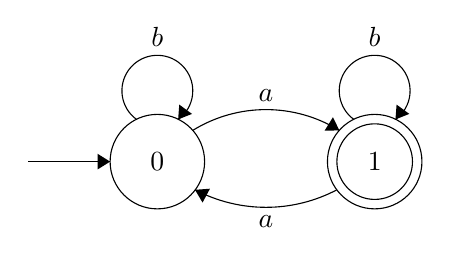
\begin{tikzpicture}[scale=0.2]
\tikzstyle{every node}+=[inner sep=0pt]
\draw [black] (27.5,-22.7) circle (3);
\draw (27.5,-22.7) node {$0$};
\draw [black] (41.3,-22.7) circle (3);
\draw (41.3,-22.7) node {$1$};
\draw [black] (41.3,-22.7) circle (2.4);
\draw [black] (19.3,-22.7) -- (24.5,-22.7);
\fill [black] (24.5,-22.7) -- (23.7,-22.2) -- (23.7,-23.2);
\draw [black] (26.177,-20.02) arc (234:-54:2.25);
\draw (27.5,-15.45) node [above] {$b$};
\fill [black] (28.82,-20.02) -- (29.7,-19.67) -- (28.89,-19.08);
\draw [black] (39.977,-20.02) arc (234:-54:2.25);
\draw (41.3,-15.45) node [above] {$b$};
\fill [black] (42.62,-20.02) -- (43.5,-19.67) -- (42.69,-19.08);
\draw [black] (29.737,-20.723) arc (121.76979:58.23021:8.856);
\fill [black] (39.06,-20.72) -- (38.65,-19.88) -- (38.12,-20.73);
\draw (34.4,-18.9) node [above] {$a$};
\draw [black] (38.905,-24.487) arc (-62.18142:-117.81858:9.653);
\fill [black] (29.89,-24.49) -- (30.37,-25.3) -- (30.84,-24.42);
\draw (34.4,-26.1) node [below] {$a$};
\end{tikzpicture}
\end{center}

\subsolution

\begin{center}
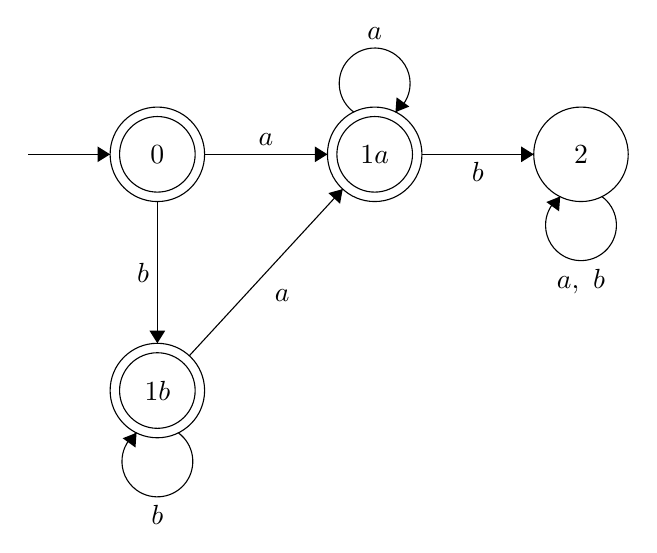
\begin{tikzpicture}[scale=0.2]
\tikzstyle{every node}+=[inner sep=0pt]
\draw [black] (27.5,-22.7) circle (3);
\draw (27.5,-22.7) node {$0$};
\draw [black] (27.5,-22.7) circle (2.4);
\draw [black] (41.3,-22.7) circle (3);
\draw (41.3,-22.7) node {$1a$};
\draw [black] (41.3,-22.7) circle (2.4);
\draw [black] (27.5,-37.7) circle (3);
\draw (27.5,-37.7) node {$1b$};
\draw [black] (27.5,-37.7) circle (2.4);
\draw [black] (54.4,-22.7) circle (3);
\draw (54.4,-22.7) node {$2$};
\draw [black] (19.3,-22.7) -- (24.5,-22.7);
\fill [black] (24.5,-22.7) -- (23.7,-22.2) -- (23.7,-23.2);
\draw [black] (39.977,-20.02) arc (234:-54:2.25);
\draw (41.3,-15.45) node [above] {$a$};
\fill [black] (42.62,-20.02) -- (43.5,-19.67) -- (42.69,-19.08);
\draw [black] (30.5,-22.7) -- (38.3,-22.7);
\fill [black] (38.3,-22.7) -- (37.5,-22.2) -- (37.5,-23.2);
\draw (34.4,-22.2) node [above] {$a$};
\draw [black] (27.5,-25.7) -- (27.5,-34.7);
\fill [black] (27.5,-34.7) -- (28,-33.9) -- (27,-33.9);
\draw (27,-30.2) node [left] {$b$};
\draw [black] (28.823,-40.38) arc (54:-234:2.25);
\draw (27.5,-44.95) node [below] {$b$};
\fill [black] (26.18,-40.38) -- (25.3,-40.73) -- (26.11,-41.32);
\draw [black] (29.53,-35.49) -- (39.27,-24.91);
\fill [black] (39.27,-24.91) -- (38.36,-25.16) -- (39.1,-25.84);
\draw (34.93,-31.66) node [right] {$a$};
\draw [black] (44.3,-22.7) -- (51.4,-22.7);
\fill [black] (51.4,-22.7) -- (50.6,-22.2) -- (50.6,-23.2);
\draw (47.85,-23.2) node [below] {$b$};
\draw [black] (55.723,-25.38) arc (54:-234:2.25);
\draw (54.4,-29.95) node [below] {$a,\mbox{ }b$};
\fill [black] (53.08,-25.38) -- (52.2,-25.73) -- (53.01,-26.32);
\end{tikzpicture}
\end{center}
\end{solution}
%% End of problems written by Erin %%
\end{document}
